% Fig. 1 of ms-10p: four coordinates for the signal of one QSP circuit.
% Compile to ../qsp_charts.pdf; included at natural size (no scaling).
\documentclass[tikz,10pt]{standalone}
\usepackage{amsmath,amssymb,bm}
\usetikzlibrary{arrows.meta,positioning,calc}
\newcommand{\R}{\mathbb{R}}
\newcommand{\T}{\mathbb{T}}
\newcommand{\TB}{\mathrm{TB}}
\newcommand{\SB}{\mathrm{SB}}
\begin{document}
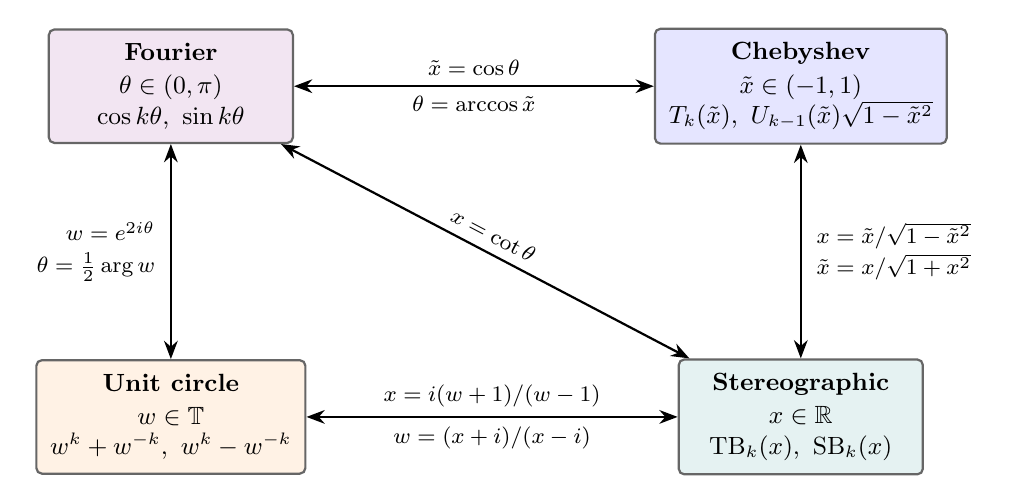
\begin{tikzpicture}[
	>=Stealth,
	every node/.style={font=\small},
	picnode/.style={
		rectangle, rounded corners=2pt, draw=black!60,
		thick, align=center, inner sep=5pt, minimum width=3.1cm
	},
	fourier/.style    ={picnode, fill=violet!10},
	chebyshev/.style  ={picnode, fill=blue!10},
	gqsp/.style       ={picnode, fill=orange!10},
	ratcheb/.style    ={picnode, fill=teal!10},
	edgelab/.style    ={font=\footnotesize, midway},
	sidelab/.style    ={font=\footnotesize, midway, align=left},
]
\node[fourier]   (F)  at (-4.0,  2.1) {%
	\textbf{Fourier} \\[1pt]
	$\theta \in (0,\pi)$ \\
	$\cos k\theta,\ \sin k\theta$};
\node[chebyshev] (C)  at ( 4.0,  2.1) {%
	\textbf{Chebyshev} \\[1pt]
	$\tilde x \in (-1,1)$ \\
	$T_k(\tilde x),\ U_{k-1}(\tilde x)\sqrt{1-\tilde x^2}$};
\node[gqsp]      (G)  at (-4.0, -2.1) {%
	\textbf{Unit circle} \\[1pt]
	$w \in \T$ \\
	$w^k+w^{-k},\ w^k-w^{-k}$};
\node[ratcheb]   (R)  at ( 4.0, -2.1) {%
	\textbf{Stereographic} \\[1pt]
	$x \in \R$ \\
	$\TB_k(x),\ \SB_k(x)$};

\draw[<->, thick] (F) -- (C)
node[edgelab, above] {$\tilde x = \cos\theta$}
node[edgelab, below] {$\theta = \arccos \tilde x$};

\draw[<->, thick] (F) -- (G)
node[sidelab, left=2pt, align=right]
{$w = e^{2i\theta}$\\[2pt] $\theta = \tfrac12\arg w$};

\draw[<->, thick] (C) -- (R)
node[sidelab, right=2pt]
{$x = \tilde x/\sqrt{1-\tilde x^2}$\\[2pt] $\tilde x = x/\sqrt{1+x^2}$};

\draw[<->, thick] (G) -- (R)
node[edgelab, above] {$x = i(w+1)/(w-1)$}
node[edgelab, below] {$w = (x+i)/(x-i)$};

\draw[<->, thick] (F) -- (R)
node[edgelab, sloped, above] {$x = \cot\theta$};
\end{tikzpicture}
\end{document}
